\documentclass[conference]{IEEEtran}
\IEEEoverridecommandlockouts
% The preceding line is only needed to identify funding in the first footnote. If that is unneeded, please comment it out.
\usepackage{cite}
\usepackage{amsmath,amssymb,amsfonts}
\usepackage{algorithmic}
\usepackage{graphicx}
\usepackage{textcomp}
\usepackage{xcolor}
% My packages start
\usepackage{orcidlink}
\usepackage{hyperref}
\usepackage{glossaries}
\usepackage{cleveref} % Reference footnotes.
\usepackage[scaled=0.9]{helvet} % Scale \textsf down
\crefformat{footnote}{#2\footnotemark[#1]#3}
\usepackage{flushend} % Balances columns on the last page.

\newacronym{jive}{JIVE}{Java Interactive Visualization Environment}
\newacronym{uml}{UML}{Unified Modeling Language}
\newacronym{ide}{IDE}{Integrated Development Environment}
\newacronym{api}{API}{Application Programming Interface}
\newacronym{mde}{MDE}{Model-driven engineering}
\newacronym{bpmn}{BPMN}{Business Process Modeling Notation}
\newcommand{\intellij}{IntelliJ IDEA}
\newcommand{\screencast}{\cite{ArtifactsICSME2022}}
% My packages end

\def\BibTeX{{\rm B\kern-.05em{\sc i\kern-.025em b}\kern-.08em
    T\kern-.1667em\lower.7ex\hbox{E}\kern-.125emX}}
\begin{document}

\title{The Visual Debugger Tool\\
{}
\thanks{}
}
\author{
    \IEEEauthorblockN{Tim Kräuter\IEEEauthorrefmark{1}\orcidlink{0000-0003-1795-0611},
    Adrian Rutle\IEEEauthorrefmark{1}\orcidlink{0000-0002-4158-1644},
    Yngve Lamo\IEEEauthorrefmark{1}\orcidlink{0000-0001-9196-1779},
    Harald König\IEEEauthorrefmark{2}\IEEEauthorrefmark{1}\orcidlink{0000-0001-6304-6311}
    }
    \IEEEauthorblockA{\IEEEauthorrefmark{1}Western Norway University of Applied Sciences, Bergen, Norway}
    \IEEEauthorblockA{\IEEEauthorrefmark{2}University of Applied Sciences, FHDW, Hannover, Germany
    \\\{tkra, aru, yla\}@hvl.no, harald.koenig@fhdw.de}
}

\maketitle
% Abstract: to be optimized.
% Introduction: done
% Tool description: more or less done check for redundancy/consistency with Tool architecture
% Tool architecture: more or less done see description.
% Related work: done
% Conclusion & future work: done
% 4 pages + 1 page of only references!

% Terminology:
% debugginf information vs. program information vs. current program state
\begin{abstract}
Debugging is an essential part of software maintenance and evolution since it allows a software developer to analyze a program step by step.
Understanding a program is required to fix potential flaws, alleviate bottlenecks, and implement new desired features.
Thus, software developers spend a large percentage of their time validating and debugging software, resulting in high software maintenance and evolution cost.
We aim to reduce this cost by providing a novel visual debugging tool to software developers to better support them during debugging.
Our debugging tool visualizes program information graphically as an object diagram and is fully integrated into the popular Java development environment \intellij{}.
\end{abstract}

\begin{IEEEkeywords}
Debugging, Visual Debugging, Visual Debugger, IntelliJ IDEA Plugin, Software Maintenance/Visualization
\end{IEEEkeywords}

\section{Introduction}
% Introduce debugging
Debugging is an essential part of software maintenance and evolution since it allows a software developer to analyze a program step by step during execution.
Nowadays, debugging tools are integrated with every modern \gls*{ide} and are generally seen as indispensable.
Debugging is used to understand program control- and data flow such that a software developer can locate and fix reported bugs or extend the program to implement new desired features.
% Motivation: Reduce the time-spent on debugging by better tooling!
Thus, debugging is crucial for software maintenance and evolution, and software developers spend between 35 and 50 percent of their time validating and debugging software \cite{odellDebuggingMindsetUnderstanding2017}.
Consequently, 50-75 percent of the total budget of software development projects is used for debugging, testing, and verification \cite{odellDebuggingMindsetUnderstanding2017}.
We aim to reduce this cost by providing a novel debugging tool to software developers to better support them during debugging.
Reduced time spent on debugging can be used to implement new features, i.e., creating value for customers.

% Debugging works on a textual representation of the software
Traditionally program information is represented in a textual manner during debugging (see \autoref{fig:variablesIntellij} in \autoref{sec:toolDescription}).
Debugging tools integrated with \glspl*{ide}, such as \intellij{} and Eclipse, show a set of top-level variables directly contained in the current program scope.
However, the desired program information is often not present in the top-level variables but spread out on lower levels of potentially different variables.
Thus, in specific scenarios, a graphical representation results in a faster and better understanding of the shown program information.
% Introduce my tool
We have developed a tool that visualizes the current program information graphically as an object diagram for better program comprehension.
Our open-source tool called the \textit{visual debugger} is integrated with \intellij{}\footnote{The tool is available through the JetBrains Marketplace \cite{VisualDebuggerIntelliJ}.}, which is the most popular Java \gls*{ide} according to the JVM Ecosystem Report 2021 \cite{JVMEcosystemReport2021}.
Compared to other tools, our visual debugger is optimized for industrial use since it is straightforward, lightweight, and can be used alongside the traditional textual debugger.
In addition, the tool's architecture enables the reuse of the visualization component in other debugging tools.
A demonstration of our tool is available online \cite{ArtifactsICSME2022}\footnote{Tool demonstration: \url{https://www.youtube.com/watch?v=lU_OgotweRk}}.

% Paper outline
The remainder of this paper is structured as follows.
We describe the visual debugger tool in detail (\autoref{sec:toolDescription}) before explaining the tool architecture (\autoref{sec:architecture}).
Finally, we discuss related work in \autoref{sec:relatedWork} and conclude in \autoref{sec:conclusion}.

\section{Tool description} \label{sec:toolDescription}
We will describe our tool using the parts list model shown in \autoref{fig:partsListModel}.
A parts list describes the decomposition of \textsf{Products} into sub-products and basic \textsf{Materials}.
Given a parts list, one can calculate the monetary cost and materials needed to construct one or more pieces of the described product\footnote{This example is inspired by the course on information systems taught by Michael Löwe at the University of Applied Sciences FHDW, Hanover.}.

\begin{figure}[h]
    \centering
    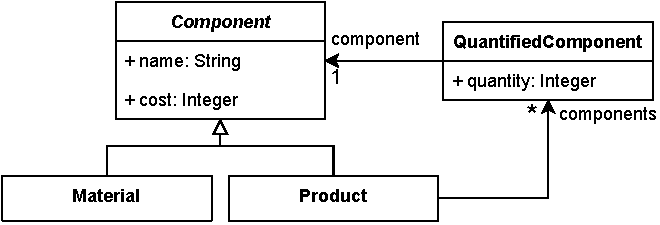
\includegraphics[width=0.48\textwidth]{images/VD-partsList-classes.pdf}
    \caption{Parts list class diagram}
    \label{fig:partsListModel}
\end{figure}

\autoref{fig:variablesIntellij} shows objects during debugging in \intellij{} conforming to the parts list model. 
The default debugger uses a textual representation for program information.

\begin{figure}[h]
    \centering
    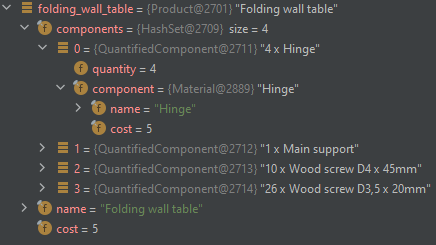
\includegraphics[width=0.4\textwidth]{images/variables.png}
    \caption{Variables during debugging in \intellij}
    \label{fig:variablesIntellij}
\end{figure}

We have unfolded the substructure of the \textsf{folding wall table} object to see its components, especially the first component, in more detail.
If one is not only interested in one attribute inside one object, but rather the whole object world using the textual representation is cumbersome.

Consequently, research on visual debugging began with the goal of fostering program comprehension.
Our tool is one of many visual debugging tools, but we aimed for excellent usability by seamlessly integrating our tool in the debugging process of the \intellij{}.
In addition, our tool is straightforward and non-intrusive, i.e., it complements textual debugging.
The goal of our tool is to make debugging during software development as efficient as possible to increase software developer productivity.

Using our visual debugger tool, we obtain the object diagram\footnote{\label{footnote:artifacts} Additional artifacts including source code, a demonstration of the visual debugger tool and a description of the Visual Debugging \acrshort*{api} can be found at \cite{ArtifactsICSME2022}.} shown in \autoref{fig:visualDebuggerVariables}, which contains the same objects and level of detail as \autoref{fig:variablesIntellij}.

\begin{figure}[h]
    \centering
    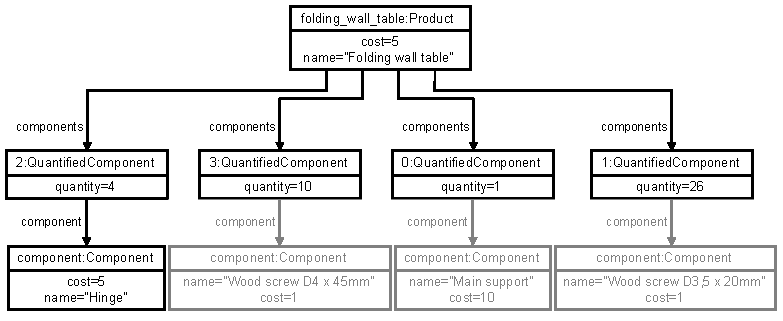
\includegraphics[width=0.48\textwidth]{images/VD-partsList-objects.pdf}
    \caption{Visual Debugger visualization comparable to \autoref{fig:variablesIntellij}}
    \label{fig:visualDebuggerVariables}
\end{figure}

% Object diagram visualization
The visual debugger tool continuously visualizes the variables in the scope of the debugging session as an \textit{object diagram}.
The visualization starts automatically when the first breakpoint is reached during debugging if the visual debugger tool is activated.
Thus, if desired, a software developer can use the visual debugger alongside the textual debugging view.
The visualization is always up to date since we listen to the events generated by a debugging session in \intellij{}.
Consequently, we update the visualization whenever a new breakpoint is reached or a user steps through the program code.

% Interaction by double clicking on an object will load all directly linked objects
Textual debugging views only show the root objects (directly referenced in the debugging session) without attributes when debugging is started.
% Initial visualization depth
Similarly, we do not visualize all objects linked to the root objects, but we allow the user to configure a \textit{visualization depth}.
The visualization depth describes how many links starting from the root objects should be followed to find objects for the initial visualization.
Afterward, one can explore objects further by double-clicking them in the visualization just as in the textual debugger.
For example, in \autoref{fig:visualDebuggerVariables}, one quantified component was explored further.

The visualization is browser-based and implemented in a standalone \textit{visualization component}, which automatically layouts the object diagram using the Eclipse Layout Kernel.
% Embedded visualizer without interaction
In addition, we provide a visualization based on PlantUML embedded in \intellij{}.
However, it is not possible to explore objects inside the embedded visualization since PlantUML provides static \gls*{uml} diagrams.

The visual debugger tool currently has 1895 unique downloads\footnote{\label{footnote:pluginStats}Last checked on 23rd of March, 2022, see \cite{VisualDebuggerIntelliJ}.} and only positive reviews.
It consists of the debugging and the visualization component, which we will describe in more detail in the tool architecture section.
Both components are open-source\cref{footnote:artifacts} and, when combined, result in the visual debugger tool.

\section{Tool architecture}  \label{sec:architecture}
First, the \textit{debugging component} integrates with \intellij{} by automatically hooking into all started debugging processes of the \gls*{ide}.
The goal of the debugging component is to obtain the current debugging information from \intellij{} and pass it on to the visualization component.
In addition, the debugging component offers a method to load detailed information for individual objects in the current debugging scope, as described earlier.
The debugging component is written in Java, and its code quality and security are continuously checked using static code analysis based on SonarCloud and unit tests.

Second, the \textit{visualization component} represents the debugging information as an object diagram to ease program understanding.
Moreover, it allows interaction to load additional debugging information for the currently shown objects.
The visualization component is \emph{browser-based} (JavaScript) and relies on a fixed \emph{Visual Debugging \gls*{api}}.
Consequently, we could implement a debugging component for a different \gls*{ide}, such as Eclipse, and reuse the visualization component.
Furthermore, the visualization component is independent of the programming language which is debugged and can potentially be reused to debug different object-oriented programming languages.

% Explain the Debugging API
The \textit{Visual Debugging \gls*{api}}\cref{footnote:artifacts} is based on \emph{WebSocket} to allow live updates about changes in the debugging information, see \autoref{fig:api}.

\begin{figure}[h]
    \centering
    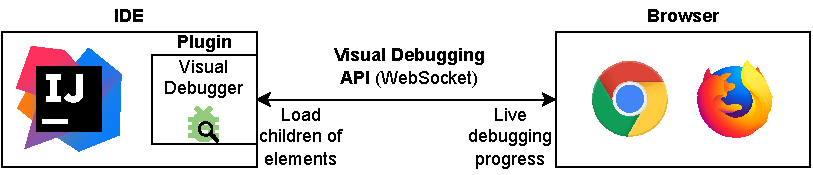
\includegraphics[width=0.488\textwidth]{images/VD-architecture.pdf}
    \caption{Communication through the Debugger API}
    \label{fig:api}
\end{figure}

Initially, a browser connects to the WebSocket server hosting the Debugger \gls*{api}, for example, the server included in our Visual Debugger plugin.
Afterward, the browser is updated in real-time about new debugging information due to debugging actions in the \gls*{ide}, such as hitting a breakpoint or jumping to the next line in the source code.
In addition, the visualization component allows a user to interact with the visualization to load all direct children of shown objects.

Debugging information, i.e., object diagram exchange, is standardized by an XSD schema \cite{ArtifactsICSME2022}.
\autoref{fig:odMetamodel} depicts the metamodel for object diagrams realized by the schema.

\begin{figure}[h]
    \centering
    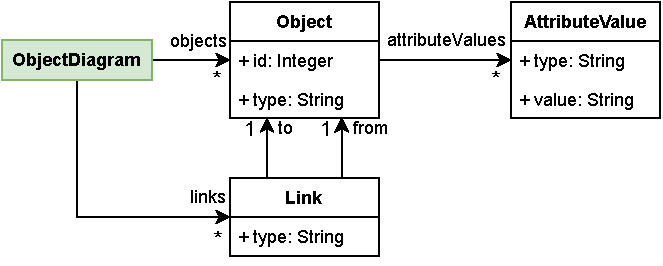
\includegraphics[width=0.488\textwidth]{images/VD-metamodel.pdf}
    \caption{Object diagram metamodel}
    \label{fig:odMetamodel}
\end{figure}

The \textsf{ObjectDiagram} is the root element in the schema (highlighted in green) and contains a set of \textsf{Objects} and \textsf{Links}.
\textsf{Objects} and \textsf{Links} have a \textsf{type}, i.e., name of a class or association.
In addition, each \textsf{Object} has a unique id provided by the debugger and a set of \textsf{attributeValues}, which have a primitive \textsf{type} and \textsf{value} modeled as strings.

Besides debugging, the visualization component provides two export features.
First, one can export object diagrams during debugging as an SVG file.
This can be useful if an undesired program state has been reached and should be documented in a bug tracking system.
Second, diagrams can be exported as an XML file that can be used to load and edit them in the object diagram modeler, for example, to show the actually desired program state.
The object diagram modeler is an open-source tool to create object diagrams in the browser, developed by the first author \cite{ObjectDiagramModeler2022}.

\section{Related work} \label{sec:relatedWork}
Visual debugging has been researched since the 90s \cite{baeza-yatesVisualDebuggingAutomatic1996, jerdingUsingVisualizationFoster1994, mukherjeaVisualDebuggingIntegrating1994, hansonSimpleExtensibleGraphical1997}, but most of the resulting tools are outdated.
We will now describe recent visual debugging tools and compare them to our tool.

% JIVE is comprehensive but the downside is that it offers too much functionality!
\textit{\gls*{jive}} is a plugin for the Eclipse \gls*{ide} \cite{czyzDeclarativeVisualDebugging2007,k.p.FiniteStateModel2021, JIVEJavaInteractive}.
It provides interactive Java program execution visualization at different levels of granularity.
The program state is visualized as a \gls*{uml} object diagram, while the call stack is represented as a \gls*{uml} sequence diagram.
\gls*{jive} is tightly coupled to the Eclipse \gls*{ide} and does not integrate with the Eclipse debugger but rather is a debugging environment on its own.
This approach is a significant difference to our tool, which integrates with the debugging tool of the \gls*{ide}.
It makes \gls*{jive} powerful but complex since it is hard to understand what is happening in the multiple views provided by \gls*{jive}.
Compared to \gls*{jive} the visual debugger tool focuses only on object diagram visualization of the current program state, which makes it lightweight and straightforward to use.
In addition, our tool decouples debugging and visualization, such that it can be adopted to different \glspl*{ide} even based on other object-oriented programming languages than Java.

% Java Visualizer
A plugin called \textit{Java Visualizer} has been developed for the \intellij{} \cite{JavaVisualizerIntelliJ}.
It visualizes the call stack and objects contained in the Java heap as a box-and-pointer diagram during a debugging session.
However, even in simple scenarios, the visualized call stacks are long since all objects from the Java heap are visualized and not only the variables in the debugging scope.
This leads to much noise in the visualization, especially if one is only interested in the current objects, i.e., the current system state.
In contrast, our tool only shows relevant information and allows users to load more information if needed.

% Debugging for distributed applications
In \cite{kochGraphicalDebuggingDistributed2015}, the authors describe a tool to debug distributed applications.
It can connect to multiple Java virtual machines and show the retrieved objects separately in an object diagram or combine the same objects from different JVMs using object identifiers or other properties.
The tool is also tightly integrated with the Eclipse \gls*{ide} and tackles the problem of debugging distributed applications, which we do not address.
However, we could not find and test the tool by ourselves.
In the future, we could incorporate these ideas by allowing multiple debugging components (one for each application) to connect to one visualization component.
The visualization component can then show the different debugging views separately or combined as described in \cite{kochGraphicalDebuggingDistributed2015}.

\textit{JAVAVIS} is a standalone tool to help students understand program execution in Java \cite{oechsleJAVAVISAutomaticProgram2002}.
It makes use of object- and sequence diagrams to represent program behavior.
However, it is not integrated with modern \glspl*{ide} such as Eclipse or \intellij{}.
Our tool can help students learn Java or object-oriented program execution in general, but we currently do not provide a sequence diagram visualization.

\section{Conclusion \& future work} \label{sec:conclusion}
% Conclude
The main contribution of this paper is the new open-source visual debugging tool, which differs from previously created tools regarding the following three aspects.
First, it is integrated with \intellij{}, a modern and popular \gls*{ide} for Java software development.
According to JVM Ecosystem Report 2021, over 70\% of JVM developers use \intellij{}  \cite{JVMEcosystemReport2021}.
In addition, the plugin received good feedback and was downloaded nearly 2000 times already\cref{footnote:pluginStats}.
Second, the visualization part of the tool is independent, such that it can be reused in other visual debugging tools.
For example, one could develop a plugin for Eclipse \gls*{ide} or Visual Studio Code in the future.
Third, we aimed for excellent usability of our tool alongside present debugging tools.
Thus, it automatically starts when debugging in \intellij{} and can be used straight away without any configuration.
Moreover, we only show a subset of the debugging information in the debugger right away and allow the user to reload more relevant information similarly to the widely adopted textual debuggers.

% Future work
We plan to improve and extend the tool in multiple ways in the future.
First, we want to do more field testing using our tool to gather feedback on the usability and features of the plugin.
This should lead to continuous improvement of the tool and greater tool use, which leads to more feedback from practitioners. 
Especially, the scalability of the tool when debugging large software systems must be investigated.
The scalability of our visual debugger should be similar to the scalability of present textual debuggers, such that our tool can be adopted in the industry.
Second, we plan to implement visual debuggers for other \glspl*{ide} and object-oriented programming languages by reusing our visualization component.
Third, we plan to reuse significant parts of our tool to debug executions of behavioral models.
Not only source code can be executed and debugged.
Behavioral models, for example, \gls*{uml} state-machines, Petri-Nets, or \gls{bpmn} processes, come with clearly defined execution semantics \cite{krauterBehavioralConsistencyHeterogeneous2021}.
% TODO: Cite ECMFA paper.
When these models are used in \gls*{mde}, it can be beneficial to execute and debug them directly.

% TODO: Comment in after acceptance and helpful feedback.
% \section*{Acknowledgment}
% We want to thank the anonymous reviewers for their valuable comments and helpful suggestions.

% TODO: check References one by one at the end!
\bibliographystyle{IEEEtran}
\bibliography{bib}

\end{document}
